\documentclass[14pt]{beamer}
\usepackage{./Estilos/BeamerUVM}
\usepackage{./Estilos/ColoresLatex}
\usepackage{circuitikz}
\usepackage{schemata}
\usetheme{Warsaw}
\usecolortheme{rose}
%\useoutertheme{default}
\setbeamercovered{invisible}
% or whatever (possibly just delete it)
\setbeamertemplate{section in toc}[sections numbered]
\setbeamertemplate{subsection in toc}[subsections numbered]
\setbeamertemplate{subsection in toc}{\leavevmode\leftskip=3.2em\rlap{\hskip-2em\inserttocsectionnumber.\inserttocsubsectionnumber}\inserttocsubsection\par}
%\setbeamercolor{section in toc}{fg=blue}
%\setbeamercolor{subsection in toc}{fg=blue}
%\setbeamercolor{frametitle}{fg=blue}
\setbeamertemplate{caption}[numbered]

\setbeamertemplate{footline}
\beamertemplatenavigationsymbolsempty
\setbeamertemplate{headline}{}


\makeatletter
\setbeamercolor{section in foot}{bg=gray!30, fg=black!90!orange}
\setbeamercolor{subsection in foot}{bg=blue!30}
\setbeamercolor{date in foot}{bg=black}
\setbeamertemplate{footline}
{
  \leavevmode%
  \hbox{%
  \begin{beamercolorbox}[wd=.333333\paperwidth,ht=2.25ex,dp=1ex,center]{section in foot}%
    \usebeamerfont{section in foot} \insertsection
  \end{beamercolorbox}%
  \begin{beamercolorbox}[wd=.333333\paperwidth,ht=2.25ex,dp=1ex,center]{subsection in foot}%
    \usebeamerfont{subsection in foot}  \insertsubsection
  \end{beamercolorbox}%
  \begin{beamercolorbox}[wd=.333333\paperwidth,ht=2.25ex,dp=1ex,right]{date in head/foot}%
    \usebeamerfont{date in head/foot} \hspace*{2em}
    \insertframenumber{} / \inserttotalframenumber \hspace*{2ex} 
  \end{beamercolorbox}}%
  \vskip0pt%
}
\makeatother

\makeatletter
\patchcmd{\beamer@sectionintoc}{\vskip1.5em}{\vskip0.8em}{}{}
\makeatother
% \usefonttheme{serif}
\usepackage[clock]{ifsym}
\DeclareSIUnit\erg{erg}
\DeclareSIUnit[number-unit-product = {\,}]\cal{cal}

\sisetup{per-mode=symbol}
\resetcounteronoverlays{saveenumi}

% Macro para agregar el logo de UVM en cada slide de la presentación

\addtobeamertemplate{frametitle}{}{%
\begin{tikzpicture}[remember picture,overlay]
\coordinate (logo) at ([xshift=-1.5cm,yshift=-0.8cm]current page.north east);
% \fill[devryblue] (logo) circle (.9cm);
% \clip (logo) circle (.75cm);
\node at (logo) {
\includegraphics[width=2.1cm]{Imagenes/logo_UVM.png}};
\end{tikzpicture}}


\title{\Large{Equilibrio} \\ \normalsize{DOMINABACH}}
\date{}

\begin{document}
\maketitle

\section*{Contenido}
\frame[allowframebreaks]{\frametitle{Contenido} \tableofcontents[currentsection, hideallsubsections]}

\section{Equilibrio}
\frame{\tableofcontents[currentsection, hideothersubsections]}
\subsection{Definición}

\begin{frame}
\frametitle{¿Qué es el equilibrio?}
En mecánica, un objeto está en \textocolor{ao}{equilibrio mecánico} cuando:
\pause
\setbeamercolor{item projected}{bg=carmine,fg=white}
\setbeamertemplate{enumerate items}{%
\usebeamercolor[bg]{item projected}%
\raisebox{1.5pt}{\colorbox{bg}{\color{fg}\footnotesize\insertenumlabel}}%
}
\begin{enumerate}[<+->]
\item La suma de todas las fuerzas que actúan sobre él es cero.
\seti
\end{enumerate}
\end{frame}
\begin{frame}
\frametitle{¿Qué es el equilibrio?}
\setbeamercolor{item projected}{bg=carmine,fg=white}
\setbeamertemplate{enumerate items}{%
\usebeamercolor[bg]{item projected}%
\raisebox{1.5pt}{\colorbox{bg}{\color{fg}\footnotesize\insertenumlabel}}%
}
\begin{enumerate}[<+->]
\conti
\item La suma de todos los momentos o torques que actúan sobre él también es cero.
\end{enumerate}
\end{frame}

\subsection{Eq. traslacional}

\begin{frame}
\frametitle{El equilibrio traslacional}
Un objeto está en \textocolor{red}{equilibrio traslacional} cuando la suma vectorial de todas las fuerzas que actúan sobre él es igual a cero.
\end{frame}
\begin{frame}
\frametitle{El equilibrio traslacional}
Esto significa que las fuerzas que actúan sobre el objeto se equilibran mutuamente y no hay una fuerza resultante que lo haga moverse en ninguna dirección.
\end{frame}
\begin{frame}
\frametitle{El equilibrio traslacional}
Matemáticamente, se puede expresar como:
\pause
\begin{align*}
\nsum F = 0
\end{align*}
\end{frame}
\begin{frame}
\frametitle{Ejemplo}
\vspace*{-1cm}
En la siguiente figura la tensión en la cuerda horizontal es de \SI{30}{\newton}. Encuentra el peso del objeto.
\pause
\begin{figure}
    \centering
    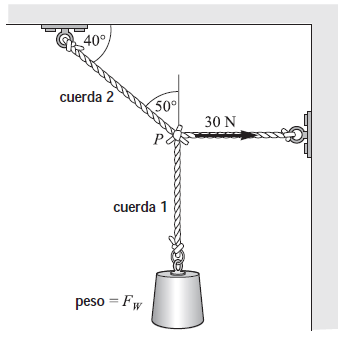
\includegraphics[scale=0.5]{Imagenes/DominaBach_01.PNG}
\end{figure}
\end{frame}
\begin{frame}
\frametitle{Descomposición de fuerzas}
Una fuerza $\va{F}$ se puede descomponer en dos partes:
\pause
\setbeamercolor{item projected}{bg=byzantine,fg=white}
\setbeamertemplate{enumerate items}{%
\usebeamercolor[bg]{item projected}%
\raisebox{1.5pt}{\colorbox{bg}{\color{fg}\footnotesize\insertenumlabel}}%
}
\begin{enumerate}[<+->]
\item $F_{x}$: la componente en la dirección del eje $x$.
\item $F_{y}$: la componente en la dirección del eje $y$.
\end{enumerate}
\end{frame}
\begin{frame}
\frametitle{Componente en la dirección $x$}
Por trigonometría se obtiene la componente $F_{x}$ cuando se conoce el ángulo $\theta$ que forma con respecto al eje $x$:
\pause
\begin{align*}
F_{x} = \cos \theta \, \abs{\va{F}}
\end{align*}
\end{frame}
\begin{frame}
\frametitle{Componente en la dirección $y$}
Mientras que la componente $F_{y}$ se obtiene:
\pause
\begin{align*}
F_{y} = \sin \theta \, \abs{\va{F}}
\end{align*}
\end{frame}
\begin{frame}
\frametitle{Condición de equilibrio}
Como se mencionó anteriormente, para que haya un equilibrio en el sistema mecánico se debe de cumplir:
\pause
\begin{align*}
\nsum F_{x} &= 0 \\[0.5em]
\nsum F_{y} &= 0
\end{align*}
\end{frame}
\begin{frame}
\frametitle{Regresando al problema}
La tensión de la cuerda $1$ es igual al peso del cuerpo que cuelga de ella.
\\
\bigskip
\pause
Por tanto $F_{T1} = F_{W}$, por lo que requiere encontrar $F_{T1} = F_{W}$.
\end{frame}
\begin{frame}
\frametitle{Diagrama de cuerpo libre}
\begin{figure}
    \centering
    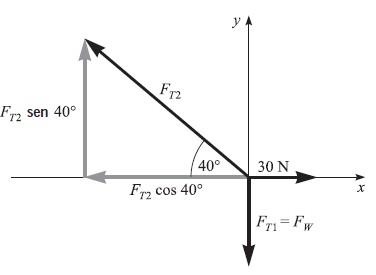
\includegraphics[scale=0.75]{Imagenes/DominaBach_02.PNG}
\end{figure}
\end{frame}
\begin{frame}
\frametitle{Componentes de la fuerza}
De las condiciones de equilibrio para las fuerzas en los ejes:
\pause
\begin{eqnarray*}
\begin{aligned}
\nsum F_{x} &= 0 \pause = \SI{30}{\newton} - F_{T2} \, \cos \ang{40} = 0 \\[0.5em] \pause
\nsum F_{y} &= 0 \pause = F_{T2} \, \sin \ang{40} - F_{W} = 0
\end{aligned}
\end{eqnarray*}
\end{frame}
\begin{frame}
\frametitle{Resolviendo las ecuaciones}
De la primera ecuación tenemos que:
\pause
\begin{eqnarray*}
\begin{aligned}
&\SI{30}{\newton} - F_{T2} \, \cos \ang{40} = 0 \\[0.5em] \pause
&F_{T2} = \dfrac{\SI{30}{\newton}}{\cos \ang{40}} = \pause \SI{39.16}{\newton}
\end{aligned}
\end{eqnarray*}
\pause
Este resultado lo sustituimos en la segunda ecuación.
\end{frame}
\begin{frame}
\frametitle{Segunda ecuación}
\begin{eqnarray*}
\begin{aligned}
&F_{T2} \, \sin \ang{40} - F_{W} = 0 \\[0.5em] \pause
&F_{W} = F_{T2} \, \sin \ang{40} = \pause (\SI{39.16}{\newton})(0.6427) = \pause \SI{25.17}{\newton}
\end{aligned}
\end{eqnarray*}
\pause
Por lo que el peso del objeto es de $F_{W} = \SI{25.17}{\newton}$
\end{frame}
\begin{frame}
\frametitle{El equilibrio traslacional}
En resumen, un objeto en equilibrio traslacional permanece en reposo o se mueve a velocidad constante en línea recta.
\end{frame}

\subsection{Equilibrio Rotacional}

\begin{frame}
\frametitle{¿Qué es el equilibrio rotacional?}
Un objeto está en equilibrio rotacional cuando la suma de todos los \textocolor{cobalt}{momentos o torques} que actúan sobre él es igual a cero.
\end{frame}
\begin{frame}
\frametitle{¿Qué es el equilibrio rotacional?}
Esto significa que las fuerzas que tienden a hacer que el objeto rote están equilibradas.
\end{frame}
\begin{frame}
\frametitle{¿Qué es el equilibrio rotacional?}
Matemáticamente, se puede expresar como:
\pause
\begin{align*}
\nsum \tau = 0
\end{align*}
\end{frame}
\begin{frame}
\frametitle{¿Qué es el equilibrio rotacional?}
En resumen, un objeto en equilibrio rotacional no experimenta una aceleración angular y no gira sobre su centro de gravedad (centro de masa).
\end{frame}
\begin{frame}
\frametitle{¿Qué es el centro de gravedad?}
El \textocolor{cadmiumgreen}{centro de gravedad (o centro de masa)} de un objeto es el punto en el cual se puede considerar que está concentrado todo su peso.
\end{frame}
\begin{frame}
\frametitle{Equilibrio rotacional}
\begin{figure}
    \centering
    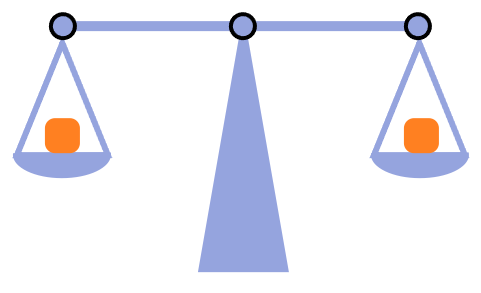
\includegraphics[scale=0.75]{Imagenes/DominaBach_03.PNG}
\end{figure}
\end{frame}
\begin{frame}
\frametitle{¿Qué es la torca?}
La \textocolor{burgundy}{torca (o momento de torsión)} $(\tau)$ alrededor de un eje, debida a una fuerza, \pause es una medida de la efectividad de la fuerza para que ésta produzca \textocolor{carmine}{una rotación} alrededor de un eje.
\end{frame}
\begin{frame}
\frametitle{Expresión para la torca}
La torca se define de la siguiente forma:
\pause
\begin{align*}
\tau = r \, F \, \sin \theta
\end{align*}
\end{frame}
\begin{frame}
\frametitle{Expresión para la torca}
\vspace*{-0.5em}
donde:
\setbeamercolor{item projected}{bg=coquelicot,fg=white}
\setbeamertemplate{enumerate items}{%
\usebeamercolor[bg]{item projected}%
\raisebox{1.5pt}{\colorbox{bg}{\color{fg}\footnotesize\insertenumlabel}}%
}
\begin{enumerate}[<+->]
\item $r$ es la distancia radial desde el eje al punto de aplicación de la fuerza.
\item $\theta$ es el ángulo agudo entre las direcciones de $r$ y de $\va{F}$.
\end{enumerate}
\end{frame}
\begin{frame}
\frametitle{La torca}
\begin{figure}
    \centering
    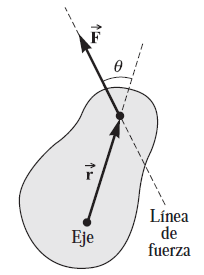
\includegraphics[scale=0.75]{Imagenes/DominaBach_04.png}
\end{figure}
\end{frame}
\begin{frame}
\frametitle{Unidades de la torca}
Las unidades de la torca son Newton metro (\unit{\newton\metre}).
\end{frame}
\begin{frame}
\frametitle{Signo de la torca}
La torca \textocolor{cordovan}{es positiva} cuando la rotación alrededor del eje es en \textocolor{cordovan}{sentido opuesto} al movimiento de las manecillas del reloj.
\begin{figure}
    \centering
    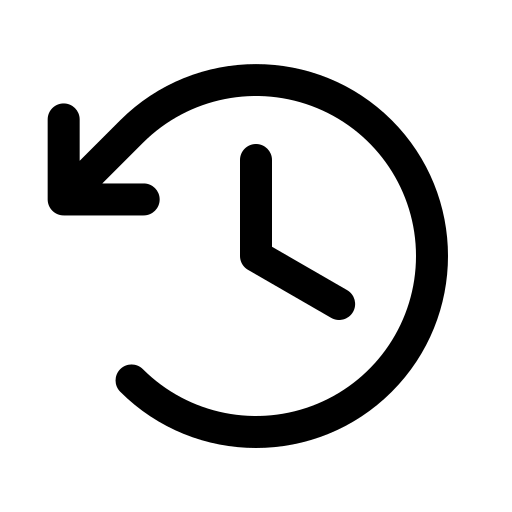
\includegraphics[scale=0.18]{Imagenes/DominaBach_05.png}
\end{figure}
\end{frame}
\begin{frame}
\frametitle{Signo de la torca}
La torca es \textocolor{darkmagenta}{negativa} cuando la rotación es en el \textocolor{darkmagenta}{mismo sentido} en que se mueven las manecillas del reloj.
\begin{figure}
    \centering
    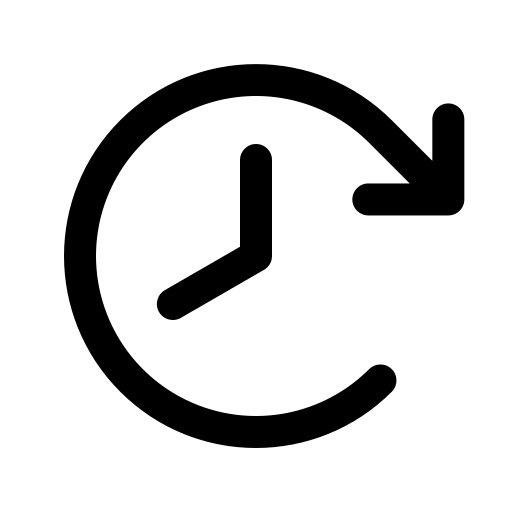
\includegraphics[scale=0.18]{Imagenes/DominaBach_06.png}
\end{figure}
\end{frame}

\section{Cuerpo rígido}
\frame{\tableofcontents[currentsection, hideothersubsections]}
\subsection{Definición}

\begin{frame}
\frametitle{¿Qué es un cuerpo rígido?}
Un \textocolor{darkmagenta}{cuerpo rígido} es aquel en el que las distancias entre sus puntos \textocolor{brown(web)}{no cambian con el tiempo}, independientemente de las fuerzas aplicadas sobre él.
\end{frame}
\begin{frame}
\frametitle{Consideraciones}
A pesar de que un cuerpo rígido \textocolor{carnelian}{puede moverse o rotar}, \pause todas sus partes se mueven o giran juntas de manera tal que la forma y las dimensiones del cuerpo no cambian.
\end{frame}
\begin{frame}
\frametitle{Análisis simplificado}
El estudio de los cuerpos rígidos es común en la mecánica debido a que simplifica muchos problemas.
\end{frame}
\begin{frame}
\frametitle{Análisis simplificado}
Por ejemplo, al considerar un objeto como un cuerpo rígido, \pause se pueden aplicar \textocolor{ao}{relaciones geométricas y trigonométricas} simples para describir su movimiento o su respuesta a las fuerzas externas.
\end{frame}
\begin{frame}
\frametitle{Ejemplos de cuerpos rígidos}
Algunos ejemplos de cuerpos rígidos son:
\setbeamercolor{item projected}{bg=carolinablue,fg=black}
\setbeamertemplate{enumerate items}{%
\usebeamercolor[bg]{item projected}%
\raisebox{1.5pt}{\colorbox{bg}{\color{fg}\footnotesize\insertenumlabel}}%
}
\begin{enumerate}[<+->]
\item Una barra metálica.
\item Una rueda de bicicleta.
\item Un bloque de madera.
\end{enumerate}
\end{frame}
\begin{frame}
\frametitle{Ejemplos de cuerpos rígidos}
Estos objetos mencionados pueden moverse o rotar, pero sus formas y dimensiones se mantienen constantes.
\end{frame}
\begin{frame}
\frametitle{Momento de inercia}
El  \textocolor{carmine}{momento de inercia} $(I)$ de un cuerpo es la medida de la inercia rotacional del cuerpo.
\end{frame}
\begin{frame}
\frametitle{Momento de inercia}
Si un objeto que puede girar libremente alrededor de un eje presenta gran dificultad para hacerlo girar, se dice que su momento de inercia alrededor de dicho eje es grande.
\end{frame}
\begin{frame}
\frametitle{Momento de inercia}
Un objeto con $I$ pequeña tiene poca inercia rotacional.
\end{frame}
\begin{frame}
\frametitle{Calculando $I$}
Si un cuerpo se considera constituido por pequeñas masas $m_{1}, m_{2}, m_{3}, \ldots $,\pause  a las distancias respectivas $r_{1}, r_{2}, r_{3}, \ldots$ a partir de un eje, \pause su momento de inercia en torno a ese eje es:
\pause
\begin{align*}
I = m_{1} \, r_{1} + m_{2} \, r_{2} + m_{3} \, r_{3} + \ldots = \nsum_{i} m_{i} \, r_{i}
\end{align*}
\end{frame}
\begin{frame}
\frametitle{Radio de giro}
Es conveniente definir un radio de giro $(k)$ para un objeto alrededor de un eje por la relación:
\pause
\begin{align*}
I = M \, k^{2}
\end{align*}
\pause 
donde $M$ es la masa total del objeto.
\end{frame}
\begin{frame}
\frametitle{Radio de giro}
En consecuencia, $k$ es la distancia a la cual se debe colocar una masa puntual $M$ desde el eje, \pause si la masa va a tener la misma $I$ que tiene el objeto.
\end{frame}
\begin{frame}
\frametitle{Torca y aceleración angular}
Una torca $\tau$ que actúa sobre un cuerpo que tiene un momento de inercia $I$ produce en él una aceleración angular $\alpha$ dada por:
\pause
\begin{align*}
\tau = I \, \alpha
\end{align*}
\end{frame}
\begin{frame}
\frametitle{Energía cinética}
La energía cinética de rotación $(EC_{r})$ de una masa cuyo momento de inercia alrededor de un eje es $I$,
y rota alrededor del eje con una velocidad angular $\omega$, es:
\pause
\begin{align*}
EC_{r} = \dfrac{1}{2} \, I \, \omega^{2}
\end{align*}
\end{frame}
\begin{frame}
\frametitle{El trabajo}
El trabajo $(W)$ efectuado sobre un cuerpo en rotación durante un desplazamiento angular $\theta$ por una torca constante $\tau$ está dado por:
\begin{align*}
W = \tau \, \theta
\end{align*}
\end{frame}
\begin{frame}
\frametitle{La potencia}
La potencia $(P)$ transmitida a un cuerpo por una torca está dada por $P$:
\begin{align*}
P = \tau \, \omega
\end{align*}
donde $\tau$ es la torca aplicada alrededor del eje de rotación y $\omega$ es la rapidez angular, alrededor del mismo eje.
\end{frame}

\section{Máquinas simples}
\frame{\tableofcontents[currentsection, hideothersubsections]}
\subsection{¿Qué son las máquinas simples?}

\begin{frame}
\frametitle{¿Qué son las máquinas simples?}
\end{frame}
\begin{frame}
\frametitle{Las máquinas simples}
Las máquinas simples son \textocolor{red}{dispositivos mecánicos} que permiten realizar trabajo con \textocolor{ao}{una menor cantidad de fuerza aplicada}.
\end{frame}
\begin{frame}
\frametitle{Las máquinas simples}
Estas máquinas están compuestas por elementos básicos y funcionan según principios físicos fundamentales.
\end{frame}
\begin{frame}
\frametitle{Las máquinas simples}
Aunque son simples en diseño, las máquinas simples son la base de muchas máquinas más complejas y se utilizan en una variedad de aplicaciones en la vida cotidiana y en la industria.
\end{frame}

\subsection{Tipos de máquinas simples}

\begin{frame}
\frametitle{Tipos de máquinas simples}
Las máquinas simples comunes incluyen:
\pause
\setbeamercolor{item projected}{bg=carmine,fg=white}
\setbeamertemplate{enumerate items}{%
\usebeamercolor[bg]{item projected}%
\raisebox{1.5pt}{\colorbox{bg}{\color{fg}\footnotesize\insertenumlabel}}%
}
\begin{enumerate}[<+->]
\item \textocolor{byzantium}{Palanca}:

Una palanca consiste en una barra rígida que puede girar alrededor de un punto de apoyo llamado fulcro.
\seti
\end{enumerate}
\end{frame}
\begin{frame}
\frametitle{La palanca}
Se utiliza para aumentar la fuerza aplicada (fuerza de entrada) o cambiar la dirección de la fuerza.
\end{frame}
\begin{frame}
\frametitle{Palanca de primer orden}
\begin{figure}
    \centering
    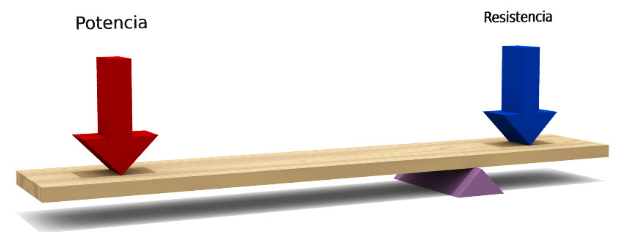
\includegraphics[scale=0.5]{Imagenes/Palanca_01.png}
\end{figure}
\end{frame}
\begin{frame}
\frametitle{Palanca de segundo orden}
\begin{figure}
    \centering
    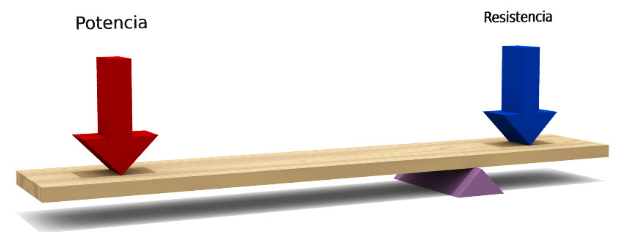
\includegraphics[scale=0.5]{Imagenes/Palanca_01.png}
\end{figure}
\end{frame}
\begin{frame}
\frametitle{Palanca de tercer orden}
\begin{figure}
    \centering
    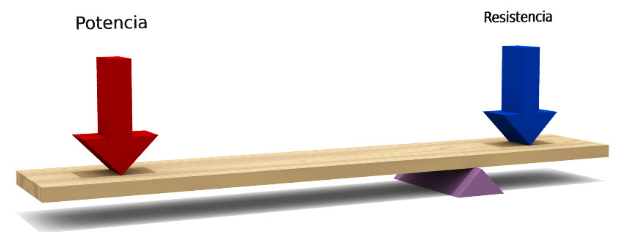
\includegraphics[scale=0.5]{Imagenes/Palanca_01.png}
\end{figure}
\end{frame}
% Ejemplos de palancas incluyen un martillo, un abrelatas y unas pinzas.
\begin{frame}
\frametitle{Tipos de máquinas simples}
\setbeamercolor{item projected}{bg=carmine,fg=white}
\setbeamertemplate{enumerate items}{%
\usebeamercolor[bg]{item projected}%
\raisebox{1.5pt}{\colorbox{bg}{\color{fg}\footnotesize\insertenumlabel}}%
}
\begin{enumerate}[<+->]
\conti
\item \textocolor{byzantium}{Polea}:

Una polea es un disco con una ranura o canal en su borde que permite que una cuerda o cable se mueva a través de ella.
\seti
\end{enumerate}
\end{frame}
\begin{frame}
\frametitle{La polea}
Se utiliza para cambiar la dirección de una fuerza aplicada y para aumentar la distancia sobre la cual se aplica la fuerza.
\end{frame}
\begin{frame}
\frametitle{La polea}
Ejemplos de poleas incluyen las poleas utilizadas en sistemas de elevación y las poleas en los sistemas de transmisión de automóviles.
\end{frame}
\begin{frame}
\frametitle{Tipos de máquinas simples}
\setbeamercolor{item projected}{bg=carmine,fg=white}
\setbeamertemplate{enumerate items}{%
\usebeamercolor[bg]{item projected}%
\raisebox{1.5pt}{\colorbox{bg}{\color{fg}\footnotesize\insertenumlabel}}%
}
\begin{enumerate}[<+->]
\conti
\item \textocolor{byzantium}{Plano inclinado}:

Un plano inclinado es una superficie plana inclinada que se utiliza para elevar objetos levantando una carga verticalmente a lo largo de una distancia horizontal más larga.
\conti
\end{enumerate}
\end{frame}
\begin{frame}
\frametitle{El plano inclinado}
Se utiliza para reducir la fuerza necesaria para levantar un objeto al aumentar la distancia sobre la cual se aplica la fuerza.
\end{frame}
\begin{frame}
\frametitle{El plano inclinado}
Ejemplos de planos inclinados incluyen rampas de acceso para sillas de ruedas y cuestas de carreteras.
\end{frame}
\begin{frame}
\frametitle{Tipos de máquinas simples}
\setbeamercolor{item projected}{bg=carmine,fg=white}
\setbeamertemplate{enumerate items}{%
\usebeamercolor[bg]{item projected}%
\raisebox{1.5pt}{\colorbox{bg}{\color{fg}\footnotesize\insertenumlabel}}%
}
\begin{enumerate}[<+->]
\conti
\item \textocolor{byzantium}{Cuña}:

Una cuña es un objeto con una o más superficies inclinadas que se utilizan para dividir, sujetar o elevar objetos.
\conti
\end{enumerate}
\end{frame}
\begin{frame}
\frametitle{La cuña}
Se utiliza para aplicar una fuerza concentrada en un área pequeña, lo que permite realizar tareas como cortar madera o clavar clavos.
\end{frame}
\begin{frame}
\frametitle{La cuña}
Ejemplos de cuñas incluyen cinceles y cuchillos.
\end{frame}
\begin{frame}
\frametitle{Tipos de máquinas simples}
\setbeamercolor{item projected}{bg=carmine,fg=white}
\setbeamertemplate{enumerate items}{%
\usebeamercolor[bg]{item projected}%
\raisebox{1.5pt}{\colorbox{bg}{\color{fg}\footnotesize\insertenumlabel}}%
}
\begin{enumerate}[<+->]
\conti
\item \textocolor{byzantium}{Torno}:

Un torno es una máquina simple que consiste en una barra o cilindro que gira alrededor de un eje. 
\seti
\end{enumerate}
\end{frame}
\begin{frame}
\frametitle{El torno}
Se utiliza para sujetar y girar objetos, lo que permite aplicar fuerza para apretar o aflojar piezas.
\end{frame}
\begin{frame}
\frametitle{El torno}
Ejemplos de tornos incluyen los utilizados en herramientas de mano y máquinas industriales.
\end{frame}
\begin{frame}
\frametitle{Tipos de máquinas simples}
\setbeamercolor{item projected}{bg=carmine,fg=white}
\setbeamertemplate{enumerate items}{%
\usebeamercolor[bg]{item projected}%
\raisebox{1.5pt}{\colorbox{bg}{\color{fg}\footnotesize\insertenumlabel}}%
}
\begin{enumerate}[<+->]
\conti
\item \textocolor{byzantium}{Tornillo}:

Un tornillo es un cilindro con una rosca en espiral alrededor de su superficie que se utiliza para sujetar y unir materiales.
\end{enumerate}
\end{frame}
\begin{frame}
\frametitle{El tornillo}
Se utiliza para convertir el movimiento de rotación en movimiento lineal, lo que permite fijar objetos juntos.
\end{frame}
\begin{frame}
\frametitle{El tornillo}
Ejemplos de tornillos incluyen los utilizados en la construcción y la fabricación de muebles.
\end{frame}
% Estas máquinas simples son componentes básicos de máquinas más complejas y se utilizan en una amplia gama de aplicaciones en la vida cotidiana y en la industria.
% \end{frame}

\end{document}